\chapter{Wprowadzenie}
W rozdziale przedstawiono cel i zakres pracy oraz podstawowe zadania i problemy wyznaczania lokalizacji. Ponadto opisano ogólną ideę stojącą za filtrami cząsteczkowymi - filtrację bayesowską. 
\section{Zadania i problemy wyznaczania lokalizacji}
Mogłoby się wydawać, iż w dzisiejszych, gdy mamy możliwość korzystania z systemu GPS, nie ma potrzeby zajmować się innymi sposobami wyznaczania lokalizacji. Jednak o ile jest to prawdą w dużej skali, jak np. gdy chce się wyznaczyć adres w mieście pod którym się znajdujemy, to gdy chcemy wyznaczyć swoją lokalizację bardziej dokładnie, np. jak to robią niektóre odkurzacze mobilne, to trzeba wykorzystać do tego dane z innych sensorów, np. lidarów. Czasami można wcale nie mieć możliwości korzystania z systemu GPS, na przykład pod wodą. Innym problemem może być poprawa już znanego przybliżonego położenia. W pracy zostaną przeanalizowane dwa problemy związane z wyznaczaniem lokalizacji:
\begin{itemize}
	\item Określanie położenia samolotu, na podstawie znanej mapy wysokościowej terenu, odczytów z wysokościomierza barometrycznego, oraz, ewentualnie, dodatkowych danych (np. odczytu z kompasu). 
	\item Określanie lokalizacji robota mobilnego, umieszczonego w ograniczonej przestrzeni z przeszkodami (ale na płaskiej powierzchni - mapa jest w dwóch wymiarach).
\end{itemize}
Mimo tego, iż są to jedynie dwa przypadki, w praktyce można je uogólnić na wile przypadków. Dla przykładu w \cite{underwater_pf} zajęto się problemem lokalizacji pod wodą, który w praktyce można rozwiązać w ten sam sposób co problem samolotu - mapa wysokości zostaje jedynie zastąpiona przez mapę głębokości.
\section{Cel pracy}
Celem pracy jest rozpoznanie możliwości zastosowania filtrów cząsteczkowych do rozwiązywania problemu lokalizacji oraz samodzielne zaimplementowanie i przebadanie kilku, uznanych arbitralnie przez autora za najciekawsze.
\section{Zakres pracy}
W zakres pracy wchodzi przegląd literatury na temat filtrów cząsteczkowych pod kątem problemów wyznaczania lokalizacji, następnie wybranie kilku rozwiązań oraz ich przebadanie. Aby było to możliwe konieczny jest także przegląd znanych narzędzi programistycznych, które mogą być zastosowane do zaimplementowania algorytmów.

\section{Idea filtracji Bayesowskiej}
Na chwilę obecną, algorytmy oparte o filtrację Bayesowską są szeroko wykorzystywane w automatyce i robotyce. W skrócie, podejście to polega na przeprowadzaniu cykli predykcji i poprawek, na podstawie rozkładu a priori oraz zbieranych w kolejnych iteracjach pomiarów, w celu wyznaczenia rozkładu a posteriori stanu. Ideę tego podejścia widać na rysunku \ref{bayes_fil_idea}. 
\begin{figure}
	\begin{center}
		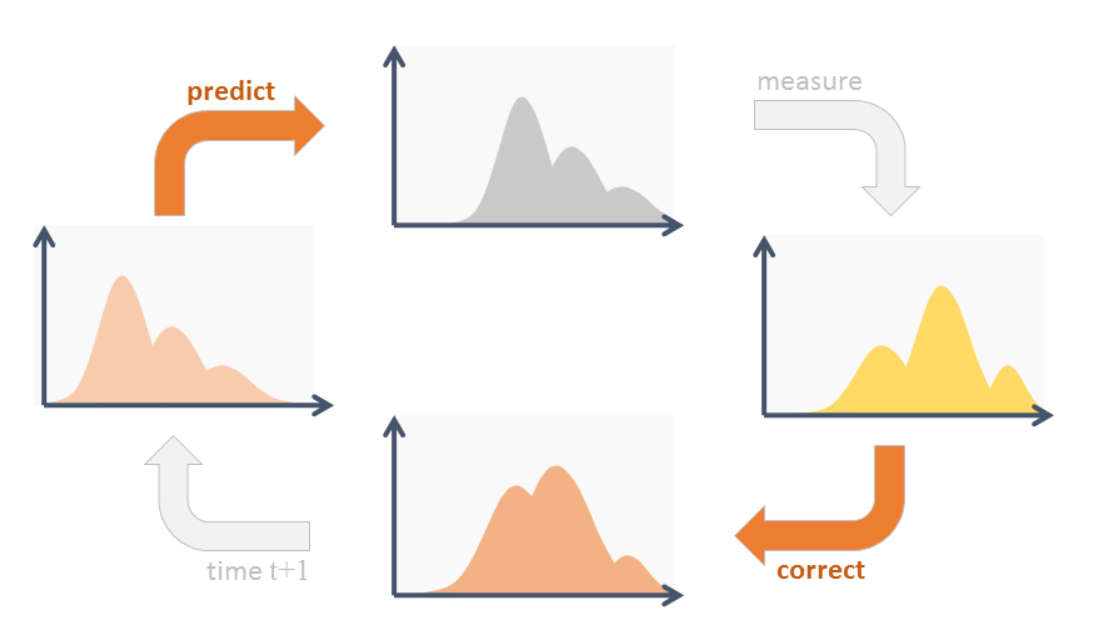
\includegraphics[width=10cm]{./predict_update.png}
		\caption{Idea filtracji Bayesowskiej. Obrazek zaczerpnięto z https://www.codeproject.com/Articles/865934/Object-Tracking-Particle-Filter-with-Ease}
		\label{bayes_fil_idea}
	\end{center}
\end{figure}
Na rysunku \ref{filtr_hier} przedstawiono hierarchię rozwiązać opartych o to podejście. Jak widać jest to bardzo duża rodzina rozwiązań, znajdujący  W pracy zostaną poruszone metody oparte o filtry cząsteczkowe.
\begin{figure}
	\begin{center}
		\includegraphics[width=10cm]{./nfg001.jpg}
		\caption{Hierarchia filtrów opartych o filtrację Bayesowską. Obrazek zaczerpnięto z \cite{prac_gui}}
		\label{filtr_hier}
	\end{center}
\end{figure}
